\chapter{Event rates and expectations for Galactic bursts}\label{ch:events}

For EMRBs to be a valuable astronomical tool we require the bursts to be loud enough to be detected; to contain sufficient information to improve our knowledge of their source systems, and to have a sufficiently high event rate that we expect to observe them over a mission lifetime. We have previously found that bursts can satisfy the first two requirements: in \chapref{param} we found Galactic bursts can be informative if the periapse distance is $r\sub{p} \lesssim 16 r\sub{g}$ and in \chapref{extragal} we found that the most promising extragalactic bursts could be informative if $r\sub{p} \lesssim 8 r\sub{g}$. We address the final requirement in this chapter.

We calculate the event rate for Galactic bursts. We only model our own Galaxy as it is the only galaxy for which we have reliable astronomical measurements of the parameters which determine the event rate. Previously, the best estimate for the event rate was given by \citet{Hopman2007}; they predicted an event rate for LISA of $\Gamma \sim 1\units{yr^{-1}}$. We follow a similar approach, but make a number of improvements: using NK waveforms to calculate the SNR and building a more detailed model for the GC's nuclear star cluster (NSC). We go on to use our event rate to define an expectation for the amount of information we could learn about the Galaxy's MBH using EMRBs.

\section{Calculating event rates}\label{sec:Rates}

Having determined how to generate a waveform and extract the information from it, we must now consider how likely it is that such a waveform would be observed. We wish to calculate the event rate for EMRBs, the probability that there is an encounter between a CO, on an orbit described by eccentricity $e$ and periapse radius $r\sub{p}$, and the MBH. To do so we must build a model to describe the distribution of COs about the MBH. The number density of stars in the six-dimensional phase space of position and velocity is described by the distribution function (DF) $f$ \citep[section 4.1]{Binney2008}. We introduce approximate forms for the DF appropriate for describing the NSC in \secref{DF}. These are calibrated using the simulations of \citet{Alexander2009}, the parameters of which, together with the others used to describe the Galactic NSC, are given in \secref{GC-Param}. Having set the distribution of COs, we explain how to convert this to an event rate in \secref{e-rp}. In \eqnref{Gamma} we give an expression that relates the event rate for an orbit $\Gamma(e,\,r\sub{p})$ and the DF. There is one final consideration before we can calculate the total event rate: that there is an inner periapsis inside of which orbits become depopulated. This is carefully explained in \secref{inner-cut}. We consider tidal disruption and collisions, which we assume truncate the DF at a finite periapsis so that the event rate inside these cut-offs is zero. We also consider GW inspiral, which we assume alters the event rate by modifying the distribution of COs away from its relaxed state. With these inner cut-offs established, we have completely defined the event rate distribution. This can then give the probability of an EMRB and the total event rates, which are presented in \secref{no-events}.

\subsection{The distribution function for the nuclear star cluster}\label{sec:DF}

Following the work of \citet{Bahcall1976, Bahcall1977}, we assume that the DF within the NSC is only a function of the orbital energy \citep{Shapiro1978}. The energy per unit mass of the orbit is
\begin{equation}
E = \dfrac{v^2}{2} - \dfrac{GM_\bullet}{r},
\end{equation}
where $v$ is the orbital velocity. The number of stars is
\begin{equation}
N = \int \dd^3r \int \dd^3v f(E).
\end{equation}
Close to the centre of the NSC, the dynamics are dominated by the influence of the MBH as it is significantly more massive than the surrounding stars. Its radius of influence is
\begin{equation}
r\sub{c} = \dfrac{GM_\bullet}{\sigma^2},
\label{eq:r_c}
\end{equation}
where $\sigma^2$ is the line-of-sight velocity dispersion \citep{Frank1976}. We assume that the mass of stars enclosed within $r\sub{c}$ is greater than $M_\bullet$, which, in turn, is much greater than the mass of a typical star $M_\star$ \citep{Bahcall1976}. We define a reference number density $n_\star$ from the enclosed mass $m_\star(r)$ such that
\begin{equation}
m_\star(r\sub{c}) = \dfrac{4\pi r\sub{c}^3}{3}n_\star M_\star.
\end{equation}
Within the NSC, the DF can be calculated using the approximation of the Fokker--Planck formalism \citep[section 7.4]{Binney2008}. The population of bound stars is evolved numerically until a steady state is reached, whilst the unbound stars form a reservoir with an assumed Maxwellian distribution. Denoting a species of star by its mass $M$, the unbound DF is
\begin{equation}
f_M(E) = \dfrac{C_M n_\star}{(2\pi\sigma_M^2)^{3/2}} \exp\left(-\dfrac{E}{\sigma_M^2}\right),\quad E > 0,
\label{eq:Unbound_DF}
\end{equation}
where $C_M$ is a normalisation constant.\footnote{$C_M$ determines the population ratios of species $M$ far from the MBH \citep{Alexander2009}.} If different stellar species are in equipartition, as assumed by \citet{Bahcall1976, Bahcall1977}, we expect
\begin{equation}
M \sigma_M^2 = M_\star \sigma_\star^2.
\end{equation}
However, if the unbound stellar population has reached equilibrium by violent relaxation, all mass groups are expected to have similar dispersions:
\begin{equation}
\sigma_M = \sigma_\star = \sigma,
\end{equation}
and we have equipartition of energy per unit mass \citep{Lynden-Bell1967}. This is assumed here following \citet{Alexander2009} and \citet{O'Leary2009}. The steady-state DF is largely insensitive to this choice \citep{Bahcall1977, Alexander2009}.

For bound orbits, the DF can be approximated as a power law \citep{Peebles1972}
\begin{equation}
f_M(E) = \dfrac{k_M n_\star}{(2\pi\sigma^2)^{3/2}}\left(-\dfrac{E}{\sigma^2}\right)^{p_M},\quad E < 0.
\label{eq:Bound_DF}
\end{equation}
The exponent $p_M$ varies depending upon the mass of the object, determining mass segregation. For a system with a single mass component $p = 1/4$ \citep{Bahcall1976, Young1977}. The normalisation constant $k_M$ reflects the relative abundances of the different species.\footnote{For a single mass population ($p = 1/4$), $k = 2 C$ gives a fit correct to within a factor of two \citep{Bahcall1976,Keshet2009}; we assume that this holds for the dominant species of stars as, although it changes slightly with $p$, variation is small compared to errors introduced by fitting a simple power law \citep{Hopman2006, Alexander2009}.}

These cusp profiles should exist if the system has had sufficient time to become gravitationally relaxed. There is current debate about whether this may be the case, both for the GC and galaxies in general. This is discussed further in \secref{tauGC}. For concreteness, we assume that a cusp has formed. If a cusp has not formed, we expect there to be a shallower core profile, with fewer objects passing close to the MBH. Our results are therefore an upper bound on possible event rates \citep{Merritt2010a,Antonini2011,Gualandris2012}. 

\subsection{Model parameters}\label{sec:GC-Param}

To describe the GC, we assume that $M_\bullet = (4.31 \pm 0.36) \times 10^6 M_\odot$ \citep{Gillessen2009} and $\sigma = (103 \pm 20)\units{km\,s^{-1}}$ \citep{Tremaine2002}. This gives an NSC radius of $r\sub{c} = (1.7 \pm 0.7)\units{pc}$. Using the results of \citet{Ghez2008} we would expect the total mass of stars in the NSC to be $m_\star(r\sub{c}) = 6.4 \times 10^6 M_\odot$, which is within $5\%$ of the value obtained similarly from \citet{Genzel2003}. This gives a reference stellar density of $n_\star = 2.8 \times 10^5\units{pc^{-3}}$.

For the distribution of COs, we use the Fokker--Planck model of \citet{Hopman2006, Hopman2006a} and \citet{Alexander2009}. This includes four species: MS stars, WDs, NSs and stellar-mass BHs. Their properties are summarised in \tabref{HA}. 
\begin{table}\footnotesize
\centering
\begin{tabular}{l D{.}{.}{2.1} D{.}{.}{1.3} D{.}{.}{1.1} D{.}{.}{1.3}} 
\toprule
  Star & \multicolumn{1}{c}{$M/M_\odot$} & \multicolumn{1}{c}{$C_M/C_\star$} & \multicolumn{1}{c}{$p_M$} & \multicolumn{1}{c}{$k_M/k_\star$\footnote{\citet*{Toonen2009}}}  \\ \midrule
  MS & 1.0 & 1 & -0.1 & 1 \\
  WD & 0.6 & 0.1 & -0.1 & 0.09 \\
  NS & 1.4 & 0.01 & 0.0 & 0.01  \\
  BH & 10 & 0.001 & 0.5 & 0.008 \\
\hline
\end{tabular}
\caption{Stellar model parameters for the Galactic NSC using the results of \citet{Alexander2009}. The MS star is used as a reference for the normalisation constants. The number fractions for unbound COs are estimates corresponding to a model of continuous star formation \citep{Alexander2005}; \citet{O'Leary2009} arrive at the same proportions.}\label{tab:HA}
\end{table}
The behaviour of the Fokker--Planck model has been verified by $N$-body simulations \citep{Baumgardt2004,Preto2010}. The spatial densities of the species as specified by the Fokker--Planck models are shown in \figref{spatial-density}. 
\begin{figure}%[ht]
  \centering
  \vspace{0.2\baselineskip}
  \includegraphics[width=0.6\textwidth]{./images/Fig_spatial_density}
    \caption{Spatial density of COs as given by the Fokker--Planck models of \citet{Alexander2009}. The distributions include both bound and unbound COs. No inner cut-offs have been applied.}   
    \label{fig:spatial-density} 
\end{figure}
The steeper power law for BHs means they segregate about the MBH. Extrapolating, they would dominate in place of MS stars for radii $r < 10^{-4}r\sub{c}$. The distributions are truncated by various processes at small radii as described in \secref{inner-cut}.

Binaries may form in the NSC, encouraged by its high stellar density \citep{O'Leary2009}. However, the binary fraction is still expected to be small \citep{Hopman2009}. Binaries are also disrupted by the MBH for periapses smaller than
\begin{equation}
r\sub{B} \simeq \left(\dfrac{M_\bullet}{M_1 + M_2}\right)^{1/3}a\sub{B},
\end{equation}
where $M_1$ and $M_2$ are the masses of the binary's components, and $a\sub{B}$ is the binary's semimajor axis, cf.\ \eqnref{Tidal} below. Thus, we ignore the possible presence of binaries.

\subsection{The event rate in terms of eccentricity and periapsis}\label{sec:e-rp}

We characterise orbits by their eccentricity $e$ and periapse radius $r\sub{p}$. The latter, unlike the semimajor axis, is always well defined regardless of eccentricity. For Keplerian orbits, the energy $E$ and angular momentum $L$ per unit mass are entirely characterised by these parameters
\begin{equation}
\label{eq:Energy_ecc}
\begin{split}
E & = -\dfrac{GM_\bullet(1 - e)}{2r\sub{p}}; \\
L^2 & = GM_\bullet(1 + e)r\sub{p}.
\end{split}
\end{equation}
The DF is defined per element of phase space: it is necessary to change variables from position and velocity to eccentricity and periapsis. We decompose the velocity into three orthogonal components: radial $v_r$, azimuthal $v_\phi$ and polar $v_\theta$. We assume that the NSC is spherically symmetric \citep{Genzel2003, Schodel2007}, therefore we are interested in the combination
\begin{equation}
v_\perp^2 = v_\phi^2 + v_\theta^2 = v^2 - v_r^2.
\end{equation}
Under this change of variables
\begin{equation}
\dd^3v = \dd v_r \dd v_\phi \dd v_\theta \rightarrow 2\pi v_\perp \,\dd v_r \,\dd v_\perp.
\end{equation}
The specific energy and angular momentum are given by
\begin{equation}
\begin{split}
E & = \dfrac{v_r^2 + v_\perp^2}{2} - \dfrac{GM_\bullet}{r}; \\
L^2 & = r^2 v_\perp^2.
\end{split}
\end{equation}
Combining these with our earlier expressions in terms of $e$ and $r\sub{p}$,
\begin{align}
v_\perp^2 = {} & \dfrac{GM_\bullet(1 + e)r\sub{p}}{r^2}, \\
v_r^2 = {} & GM_\bullet\left[\dfrac{2}{r} - \dfrac{(1 - e)}{r\sub{p}} - \dfrac{(1 + e)r\sub{p}}{r^2}\right].
\end{align}
From the latter we can verify that the turning points of an orbit occur at
\begin{equation}
r = r\sub{p}, \quad \dfrac{1+e}{1-e}r\sub{p};
\end{equation}
the periapse is the only turning point for orbits with $e > 1$. Since we now have expressions for $\{v_r, v_\perp\}$ in terms of $\{e, r\sub{p}\}$, we can 
calculate the Jacobian
\begin{equation}
\left|\dfrac{\partial(v_r, v_\perp)}{\partial(e, r\sub{p})}\right| = \recip{2v_rv_\perp}\dfrac{e}{r\sub{p}}\left(\dfrac{GM_\bullet}{r}\right)^2.
\end{equation}
Using this, we may
rewrite our velocity element as
\begin{equation}
\dd^3v \rightarrow \dfrac{\pi e}{v_r r\sub{p}}\left(\dfrac{GM_\bullet}{r}\right)^2\,\dd e \,\dd r\sub{p}.
\end{equation}
As a consequence of our assumed spherical symmetry, 
the volume element is
\begin{equation}
\dd^3r \rightarrow 4\pi r^2 \,\dd r.
\end{equation}
Thus, 
the phase space volume element can be expressed as
\begin{equation}
\dd^3r\dd^3v \rightarrow \dfrac{4\pi^2(GM_\bullet)^2e}{v_r r\sub{p}}\,\dd r\,\dd e \,\dd r\sub{p}.
\end{equation}
The number of stars in an element $\dd r\,\dd e\,\dd r\sub{p}$ is
\begin{equation}
n(r, e, r\sub{p})\,\dd r\,\dd e\,\dd r\sub{p} = \dfrac{4\pi^2(GM_\bullet)^2e}{v_r r\sub{p}}f(E)\,\dd r\,\dd e\,\dd r\sub{p}.
\end{equation}

From this, we can construct the expected number of stars on orbits defined by $\{e, r\sub{p}\}$. The number of stars found in a small radius range $\delta r$ with given orbital properties is
\begin{equation}
n(r, e, r\sub{p})\delta r = N(e, r\sub{p}; r)\dfrac{\delta t}{P(e, r\sub{p})},
\end{equation}
where $N(e, r\sub{p}; r)$ is the total number of stars with orbits given by $\{e, r\sub{p}\}$ defined at $r$, $\delta t$ is the time spent in $\delta r$ and $P(e, r\sub{p})$ is the period of the orbit. We defer the definition of this time for unbound orbits for now. The time spent in the radius range is
\begin{equation}
\delta t = 2\dfrac{\delta r}{v_r},
\end{equation}
where the factor of two accounts for inward and outward motion. Hence,
\begin{align}
N(e, r\sub{p}; r) = {} & \recip{2} v_r P(e, r\sub{p}) n(r, e, r\sub{p}) = \dfrac{2\pi^2(GM_\bullet)^2 e P(e, r\sub{p})}{r\sub{p}}f(E).
\end{align}
The right hand side is independent of position, subject to the constraint that the radius is in the allowed range for the orbit $r\sub{p} \leq r \leq (1+e)r\sub{p}/(1-e)$, and so $N(e, r\sub{p}) \equiv N(e, r\sub{p}; r)$. This is a consequence of the DF being dependent only upon a constant of the motion.\footnote{See \citet{Bahcall1976} equation 9 for a similar result.}

If a burst of radiation is emitted each time a star passes through periapse, the event rate for burst emission from orbits with parameters $\{e, r\sub{p}\}$ is given by
\begin{align}
\Gamma(e, r\sub{p}) = {} & \dfrac{N(e, r\sub{p})}{P(e, r\sub{p})} = \dfrac{2\pi^2(GM_\bullet)^2 e}{r\sub{p}}f(E).
\label{eq:Gamma}
\end{align}
The orbital period drops out from the calculation, so we do not have to worry about an appropriate definition for unbound orbits.

%From the event rate we may define a probability of seeing a given number of events subject to the assumption they are uncorrelated: it is given by the Poisson distribution. The probability of there being $r$ events is
%\begin{equation}
%\Pr(r|\Gamma(e, r\sub{p})) = \dfrac{\Gamma^r\exp(-\Gamma)}{r!}.
%\end{equation}
%The probability of there being a burst from an orbit with periapse $r\sub{p}$ and eccentricity $e$ is hence
%\begin{equation}
%\Pr(r \neq 0|\Gamma(e, r\sub{p})) = 1 - \Pr(r = 0|\Gamma(e, r\sub{p})).
%\end{equation}

%To estimate the expectation of a quantity across all orbits we use
%\begin{equation}
%\left\langle X\right\rangle = \sum\sub{R} \int_0^\infty \dd e \int_0^\infty \dd r\sub{p} X(r;r\sub{p},e)\Pr(r|\Gamma(e, r\sub{p})).
%\end{equation}
%Since the probability decays rapidly for large $r$, we may truncate the sum to give the required level of accuracy,

To generate a representative sample for the orbital parameters $e$ and $r\sub{p}$, we use $\Gamma(e, r\sub{p})\dd e\, \dd r\sub{p}$ as the rate for a Poisson distribution.

The total event rate can be found by integrating $\Gamma(e,\,r\sub{p})$, but before we can do this we must set the limits of the integral. The maximum periapse is set by the limit of detectability. It is particular to the detector. The inner periapse is set by physical processes. These are explained in the following section.

\subsection{The inner cut-off}\label{sec:inner-cut}

From \eqnref{Gamma} we see that the event rate is highly sensitive to the smallest value of the periapsis. Ultimately, the orbits cannot encroach closer to the MBH than its last stable orbit. This depends upon the spin of the MBH, but is of the order of its Schwarzschild radius. Before we reach this point, there are other processes that may intervene to deplete the orbiting stars. Our treatment of these is approximate, but should produce reasonable estimates. We consider three processes: tidal disruption by the MBH (\secref{Tidal}), GW inspiral (\secref{GW-in}) and collisional disruption (\secref{Collision}). Tidal disruption imposes a definite (albeit approximate) cut-off, while the others use statistical arguments. For these methods, we will need to define a reference time-scale for relaxation. This is done in \secref{Relax}, with further details found in \chapref{relax}.

The calculated inner cut-offs for the four stellar species across the range of bound orbits are shown in \figref{Cuts}.
\begin{figure}%[ht]
\centering
   \subfigure[{MS stars}]{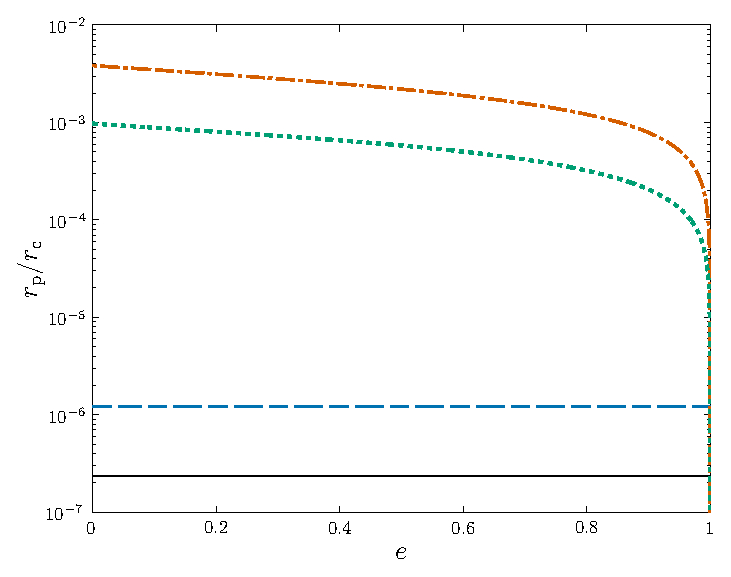
\includegraphics[width=0.475\textwidth]{./images/Fig_Inner_cut_1.eps}} \quad 
   \subfigure[{WDs}]{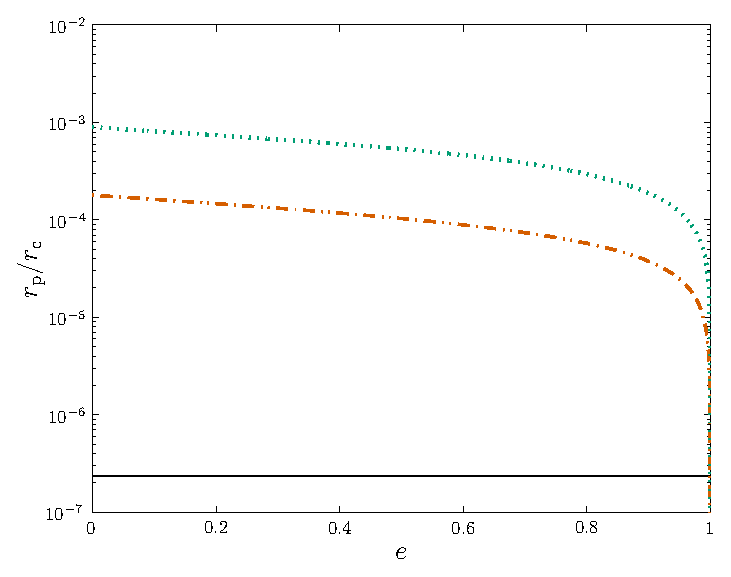
\includegraphics[width=0.475\textwidth]{./images/Fig_Inner_cut_2.eps}} \\
   \subfigure[{NSs}]{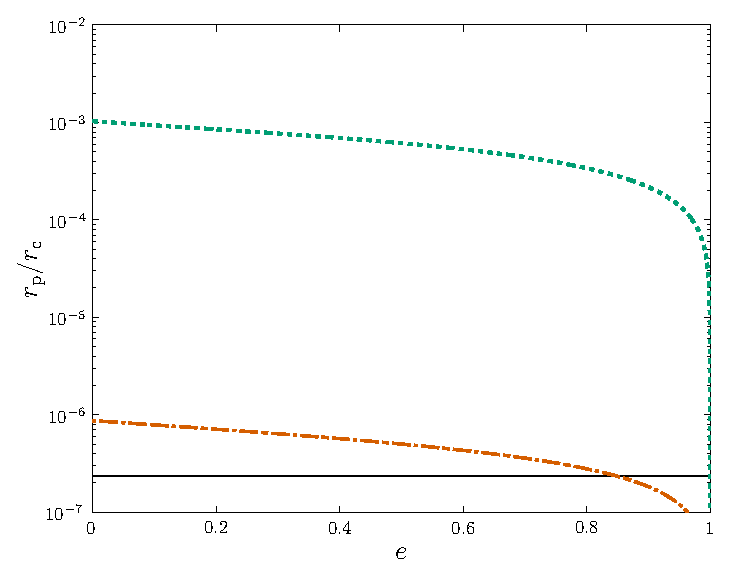
\includegraphics[width=0.475\textwidth]{./images/Fig_Inner_cut_3.eps}} \quad
   \subfigure[{BHs}]{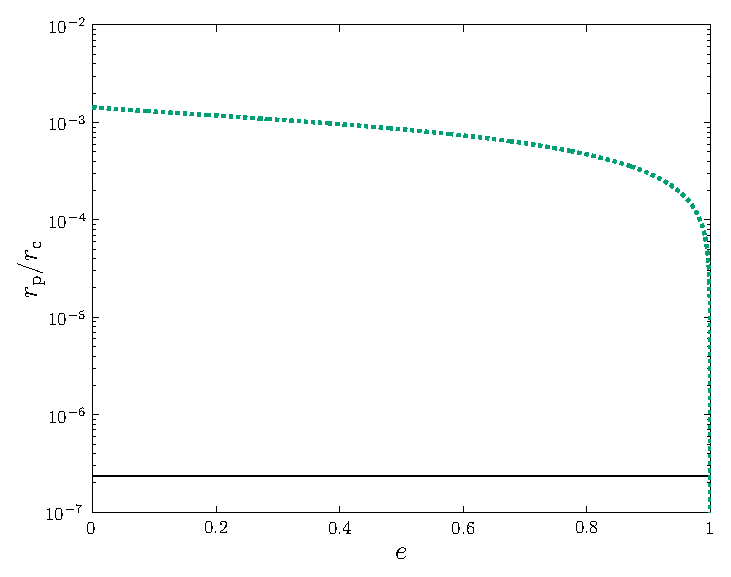
\includegraphics[width=0.475\textwidth]{./images/Fig_Inner_cut_4.eps}}
\caption{Inner cut-off radii for the GC as a function of eccentricity. The solid line sows the Schwarzschild radius of the MBH; this gives an indication of the innermost possible orbit, which actually varies with MBH spin as well as orbital eccentricity and inclination. The dashed line shows the tidal radius, which is a hard cut-off inside of which there should be no undisrupted stars. The dot--dashed line shows the collisional cut-off, which is a statistical cut-off inside of which we do not expect any stars. The dotted line shows the transition to the GW-dominated inspiral regime; inside of this we expect inspiralling stars in place of the relaxed distribution.}\label{fig:Cuts}
\end{figure}
The tidal and collisional disruption cut-offs are hard boundaries, inside of which we assume that there are no bursting sources. The transition to the GW inspiral dominated regime marks the end of the relaxed distribution of stars; inside of this there are only inspiralling stars.

\subsubsection{Tidal disruption}\label{sec:Tidal}

Tidal forces from the MBH can disrupt stars. This occurs at the tidal radius
\begin{equation}
r\sub{T} \simeq \left(\dfrac{M_\bullet}{M}\right)^{1/3}R_M,
\label{eq:Tidal}
\end{equation}
where $R_M$ is the radius of the star \citep{Hills1975, Rees1988, Kobayashi2004}.\footnote{See \citet{Kesden2012} for a general relativistic treatment.} Any star on an orbit with $r\sub{p} < r\sub{T}$ is disrupted in the course of its orbit. Parameterizing orbits by their periapsis allows us to easily determine which stars should be disrupted. We do not include the full effects of the loss cone \citep{Frank1976, Lightman1977, Cohn1978} as these were not incorporated into the Fokker--Planck calculations \citep{Hopman2009}.\footnote{The loss cone is a region in velocity space where orbits are depleted because stars are disrupted more rapidly than they can be replenished by two-body scattering and is discussed in \apref{loss-cone}.} The effect of the loss cone should be small, only modifying the DF by a logarithmic term \citep{Lightman1977, Bahcall1977, Cohn1978}. Its effects are diluted by resonant relaxation \citep{Hopman2007,Toonen2009,Merritt2011}. Furthermore, the loss cone could be refilled by the wandering within the NSC of the MBH because of perturbations from the inhomogeneities in the stellar potential \citep{Sigurdsson1997,Chatterjee2002,Merritt2007}.

Tidal disruption is significant for MS stars since they are least dense: calculated in this way, only MS stars are tidally disrupted outside of the MBH's event horizon \citep{Sigurdsson1997}. The tidal radius defines the cut-off for periapsis of high eccentricity ($e \gtrsim 1$) orbits \citep{Lightman1977}.

\subsubsection{Relaxation time-scale}\label{sec:Relax}

The motion of a star is determined not only by the dominant influence of the central MBH, but also by the other stars. The gravitational potential of the stars may be split into two components: a smooth background representing the average distribution of stars, and statistical fluctuations from random deviations in the stellar distribution because of individual stellar motions. The former only contributes to the stars' orbits: we neglect this since we are more interested in the influence of the MBH. The latter may be approximated as a series of two-body encounters. These lead to scattering, in a manner much like Brownian motion \citep{Bekenstein1992,Maoz1993,Nelson1999}.

The two-body interactions mostly lead to small deflections. Over time, these may accumulate into a significant change in the dynamics. The relaxation time-scale characterises the time taken for this to happen \citep[section 1.2.1]{Binney2008}. It therefore quantifies the time over which an orbit may be repopulated by scattering.

There are a variety of different methods used to define a relaxation time-scale. We follow the classic treatment of \citet[chapter 2]{Chandrasekhar1960}, adapting from a Maxwellian distribution of velocities to one derived from the DFs, equations (\ref{eq:Unbound_DF}) and (\ref{eq:Bound_DF}); this makes the model self-consistent. The derivation of the relaxation time-scale is found in \chapref{relax}, since it is too involved to include here. An average time-scale for the entire system $\overline{\tau\sub{R}}$ is defined in \eqnref{system-relax}, and an average for an orbit $\left\langle\tau\sub{R}\right\rangle$ is defined in \eqnref{orbital-relax}. 

Two-body interactions lead to diffusion in both energy and angular momentum. When considering a single (bound) orbit, over a relaxation time-scale the energy changes by order of itself while the angular momentum changes by the angular momentum of a circular orbit with that energy $L\sub{circ}(E)$ \citep{Lightman1977, Rauch1996, Hopman2005, Madigan2011}:\footnote{$L\sub{circ}(E)$ is the maximum value for orbits of that energy.}
\begin{equation}
\left(\dfrac{\Delta E}{E}\right)^{2} \approx \left[\dfrac{\Delta L}{L\sub{circ}(E)}\right]^{2} \approx \dfrac{t}{\tau\sub{R}}.
\label{eq:diffuse-relax}
\end{equation}
We may define another angular momentum relaxation time-scale as the time taken for the angular momentum to change by order of itself \citep{Merritt2011}
\begin{align}
\tau_L = {} & \left[\dfrac{L}{L\sub{circ}(E)}\right]^2\tau\sub{R} = \left(1 - e^2\right) \tau\sub{R}.
\label{eq:J-time}
\end{align}
This can be much shorter than the energy relaxation time-scale: diffusion in angular momentum can proceed more rapidly than diffusion in energy.

\subsubsection{Gravitational wave inspiral}\label{sec:GW-in}

Stars orbiting the MBH continually emit gravitational radiation; this carries away energy and angular momentum, causing the stars to inspiral. Using the analysis of \citet{Peters1963} and \citet{Peters1964} for Keplerian binaries, it is possible to define a characteristic inspiral time-scale from the rate of change of energy. For consistency with the relaxation time-scale, we define this as \citep{MiraldaEscude2000, Merritt2011}
\begin{equation}
\tau\sub{GW} \simeq E\left\langle\diff{E}{t}\right\rangle^{-1},
\label{eq:tGW-def}
\end{equation}
where the term in angular brackets is the orbit-averaged rate of energy radiation. Using \eqnref{Energy_ecc} and equation 16 of \citet{Peters1963},
\begin{align}
\tau\sub{GW} \simeq {} & \dfrac{5}{64}\dfrac{c^5r\sub{p}^4}{G^3MM_\bullet\left(M + M_\bullet\right)}\dfrac{(1+e)^{7/2}}{(1-e)^{1/2}}\left(1+\dfrac{73}{24}e^2 + \dfrac{37}{96}e^4\right)^{-1} \\
 \approx {} & \dfrac{5}{64}\dfrac{c^5r\sub{p}^4}{G^3MM_\bullet^2}\dfrac{(1+e)^{7/2}}{(1-e)^{1/2}}\left(1+\dfrac{73}{24}e^2 + \dfrac{37}{96}e^4\right)^{-1}.
\end{align}
For comparison, the total time taken for the inspiral, if undisturbed, is given in \apref{Bound}.

The time-scale associated with changes in angular momentum is \citep{Peters1964}
\begin{align}
\tau_{\mathrm{GW},\, L} \simeq {} & L\left\langle\diff{L}{t}\right\rangle^{-1} \\
 \simeq {} & \dfrac{5}{32}\dfrac{c^5r\sub{p}^4}{G^3MM_\bullet\left(M + M_\bullet\right)}\dfrac{(1+e)^{5/2}}{(1-e)^{3/2}}\left(1+\dfrac{7}{8}e^2\right)^{-1} \\
 \approx {} & \dfrac{5}{32}\dfrac{c^5r\sub{p}^4}{G^3MM_\bullet^2}\dfrac{(1+e)^{5/2}}{(1-e)^{3/2}}\left(1+\dfrac{7}{8}e^2\right)^{-1}.
\end{align}
This is always greater than the energy time-scale; hence, we only consider changes in energy from GW emission as important for evolution of the system \citep{Hopman2005}.

Unbound stars only undergo a single periapse passage and only radiate one burst of radiation; we therefore neglect any evolution in their orbital parameters.\footnote{Changes are only important for very high eccentricity orbits (\apref{Unbound}). These are high energy and are exponentially suppressed because of the Boltzmann factor in \eqnref{Unbound_DF}.}

The $(1-e)^{-1/2}$ dependence of $\tau\sub{GW}$ for bound orbits connects the two regimes. The rate of change of energy goes to zero as a consequence of assuming the orbital parameters do not change over the course of an orbit. It is a valid approximation since the large mass-ratio ensures a slow evolution of the system (\apref{Unbound}).

When comparing with the relaxation time-scale we are comparing rates of change, with the shorter time-scale highlighting the more rapid process that dominates the evolution \citep{Amaro-Seoane2007}. We therefore compare $\tau\sub{GW}$ with the orbital relaxation time-scale $\tau_L$ \citep{Merritt2011}. Orbits with $\tau\sub{GW} < \tau_L$ become depleted by GW emission faster than they are replenished by scattering. The cusp does not extend to these orbits. Yet, these orbits are not totally depopulated as an object may pass through during its inspiral from greater periapse and eccentricity. In their calculations, \citet{Hopman2007} did not include these inspiralling COs as potential burst sources. We calculate the density of COs in this region by following the evolution of inspirals beginning at the inner edge of the cusp (where the two time-scales are equal), weighting by the rate of change of the periapse and eccentricity in each element of $e$--$r\sub{p}$ space \citep{Peters1964}. The net effects are that the high-eccentricity distributions of MS stars, WDs and NSs are relatively unchanged from their cusp states, but the BH distribution is significantly depleted.

\subsubsection{Collisions}\label{sec:Collision}

As a consequence of the high densities in the NSC, stars may undergo a large number of close encounters with other stars \citep{Cohn1978}. These may lead to their destruction. MS stars, WDs and NSs may be pulled apart by tidal forces if they stray too close to a more massive object. As MS stars are diffuse, they would not tidally disrupt another star \citep{Murphy1991,Freitag2005}. Close encounters would result in some mass transfer; the cumulative effect of $20$--$30$ grazing collisions could destroy an MS star \citep{Freitag2006}. The number of collisions a star undergoes in a time interval $\delta t$ is
\begin{equation}
\delta K = n(r) A v(r,e,r\sub{p})\delta t,
\end{equation}
where $A$ is the collisional cross-sectional area. For tidal disruption, where the encounter is with a collapsed object (WD, NS or BH), we set $A = \pi r_{\mathrm{T},\,{M'}}^2$, where $r_{\mathrm{T},\,{M'}}$ is the appropriate tidal radius,
\begin{equation}
r\sub{T,\,{M'}} \simeq \left(\dfrac{M'}{M}\right)^{1/3}R_M
\end{equation}
for a CO of mass $M'$. For collisions between MS stars, the cross-sectional area is simply the geometric $A = \pi R_\star^2$.\footnote{Here we assume that the relative velocity of the colliding stars is much greater than the escape velocity of the star so we may neglect the effects of gravitational focusing.}

For circular orbits, we can find the radius at which collisions lead to disruptions by setting $\delta K = 1$ for tidal disruption or $\delta K = 20$ for grazing collisions, and $\delta t = \overline{\tau_{\mathrm{R},\,M}}$. We use the system average relaxation time-scale for the species of mass $M$ as this is the time over which stars are replenished from the reservoir. For non-circular orbits, we must consider variation with position. Using $\delta r = v_r \delta t$, and then converting to an integral, for bound orbits
\begin{equation}
K = 2 A \dfrac{\overline{\tau_{\mathrm{R},\,M}}}{P(r\sub{p},e)}\intd{r\sub{p}}{(1+e)r\sub{p}/(1-e)}{n(r)\dfrac{v(r,e,r\sub{p})}{v_r(r,e,r\sub{p})}}{r},
\label{eq:collision-K}
\end{equation}
where $P$ is the period of the orbit. Again we set $K = 1$ or $K = 20$, and then numerically solve \eqnref{collision-K} to find the orbits for which stars will be disrupted within $\overline{\tau_{\mathrm{R},\,M}}$. For unbound orbits we are only interested in stars that would become disrupted before their periapse passage, so
\begin{equation}
K = A \intd{r\sub{p}}{r\sub{c}}{n(r)\dfrac{v(r,e,r\sub{p})}{v_r(r,e,r\sub{p})}}{r},
\end{equation}
assuming that the stars in the reservoir external to the NSC are unlikely to undergo close collisions.

Orbits within the collisional cut-off are assumed to be depopulated and do not contribute to the event rate. Our treatment is similar to that of \citet{Hopman2007}, but they only considered collisions between MS stars. Collisions provide the cut-off for bound MS stars and are significant for bound WDs.

\section{Number of events}\label{sec:no-events}

\subsection{Galactic event rate}

As a first approximation for the number of events expected in a $2\units{yr}$ mission lifetime, we numerically integrated the event rate. This estimate is denoted by $\mathcal{N}_{2\units{yr}}\super{int}$. The lower limit on $r\sub{p}$ was set to be the largest of the tidal cut-off, the collisional cut-off or the MBH's Schwarzschild radius.\footnote{The transition to the GW inspiral regime is not a cut-off, but reflects a change in the form of the stellar distribution; hence, it is not included amongst the other inner periapses as a lower limit.} The Schwarzschild radius $r\sub{S} = 2 r\sub{g}$ is used as a proxy for an averaged innermost orbit's periapse; the innermost parabolic orbit for non-spinning MBHs has $r\sub{p} = 4r\sub{g}$, and the innermost parabolic orbit for a maximally spinning MBH has $r\sub{p} = r\sub{g}$ for a prograde equatorial orbit and $r\sub{p} = (3 + 2\sqrt{2})r\sub{g}$ for a retrograde equatorial orbit. The upper limit was the detection threshold as determined from \eqnref{SNR-power-law}. The lower bound on eccentricity was set to $0.9$, below which we do not trust the parabolic approximation for burst waveforms; since the DF decays exponentially with eccentricity for unbound orbits, the upper limit does not influence our results.

To obtain a more accurate estimate, we performed $2 \times 10^4$ mission realisations. For each mission, we randomly selected a set of parameters to describe the MBH, and then picked orbits with probabilities defined by their event rates. The orbital position of the LISA detector was also chosen randomly. The SNRs of the resulting bursts were calculated and a detection was recorded if $\rho > 10$. By averaging the number of events per mission, we can estimate the expected number of bursts we could detect. This is denoted by $\mathcal{N}_{2\units{yr}}\super{run}$.

The calculated numbers of events are shown in \tabref{Rates}. 
\begin{table}\footnotesize
\centering
  \begin{tabular}{l D{,}{\,\times\,}{3.4} D{,}{\,\times\,}{3.4}}
  \toprule
  Star & \multicolumn{1}{c}{$\mathcal{N}_{2\units{yr}}\super{int}$} & \multicolumn{1}{c}{$\mathcal{N}_{2\units{yr}}\super{run}$} \\ \midrule
  MS & 9.5,10^{-4} & 1.3,10^{-3} \\
  WD & 1.0,10^{-2} & 1.0,10^{-2} \\
  NS & 5.0,10^{-1} & 5.0,10^{-1}  \\
  BH & 1.2,10^{0} & 1.2,10^{0} \\
  \midrule
  Total & 1.7,10^{0} & 1.7,10^{0} \\
  \bottomrule
\end{tabular}
  \caption{Expected number of events per $2\units{yr}$ LISA mission. $\mathcal{N}_{2\units{yr}}\super{int}$ is an estimate using the average SNR--periapsis scaling, \eqnref{SNR-power-law}, and $\mathcal{N}_{2\units{yr}}\super{run}$ is calculated by averaging results from $2 \times 10^4$ mission realisations.}\label{tab:Rates}
\end{table}
The two approaches are in good agreement indicating that the average relation \eqnref{SNR-power-law} is sufficiently accurate for this type of calculation, and that the Schwarzschild radius is a reasonable absolute inner cut-off averaged over all MBH spins. The total number of events per mission is plotted in \figref{Event-no}. 
This is consistent with being Poisson distributed as expected.
\begin{figure}%[ht]
\centering
   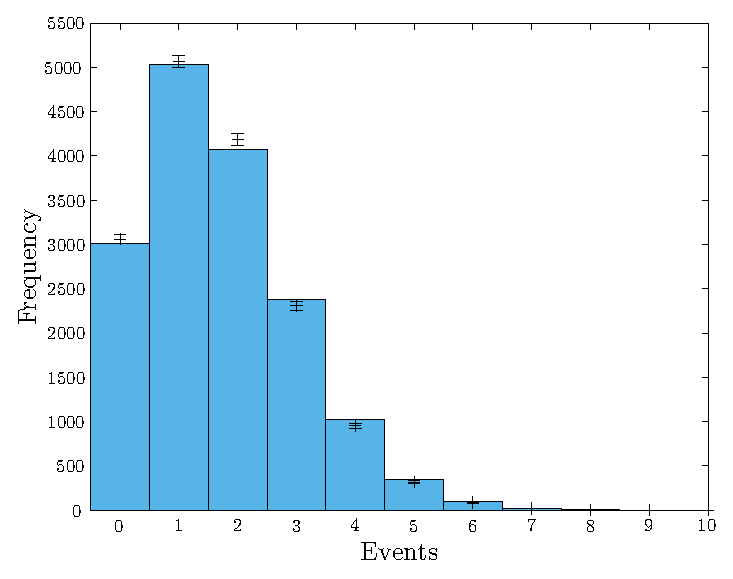
\includegraphics[width=0.6\textwidth]{./images/Fig_Total_event_hist}
\caption{Calculated number of detectable EMRBs over a $2\units{yr}$ LISA mission. The histogram shows the number of events for $2 \times 10^4$ realisations. The points show a Poisson distribution with a mean set by $\mathcal{N}_{2\units{yr}}\super{int}$.}
\label{fig:Event-no}
\end{figure}
Only BHs and NSs contribute to the event rate significantly. Only MS stars have a non-negligible (relative) contribution from unbound orbits. The event rates are not high, but there is an $\sim 4/5$ ($81\%$) chance of observing at least one burst in a mission.

The overall rates are similar to those presented in \citet{Hopman2007}. The MS rate is lower because of a larger collisional cut-off. This also influences the WD rate, but the overall rate is little changed. The NS rate is enhanced because of the inclusion of bursts from inspiralling objects. The physics for BHs is least changed; the (small) difference in the event rate is partly a consequence of our more realistic SNRs.

The distribution of SNRs for the set of detectable ($\rho > 10$) bursts is shown in \figref{SNR-hist}.
\begin{figure}%[ht]
\centering
   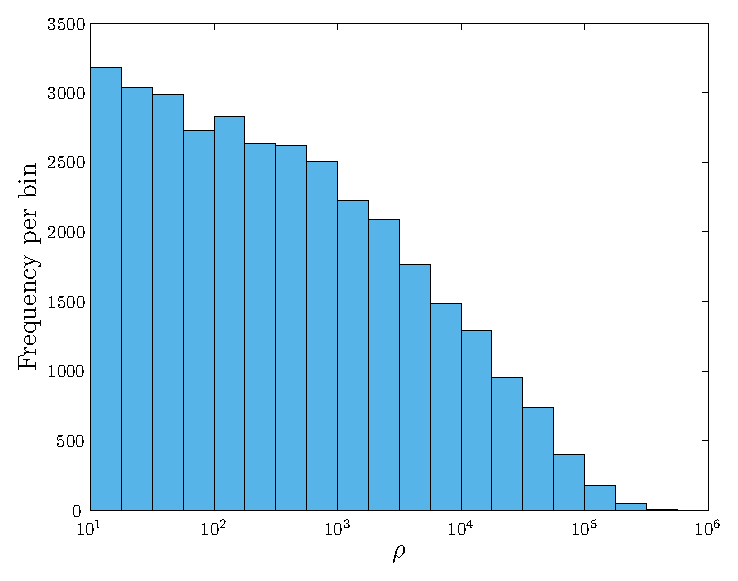
\includegraphics[width=0.6\textwidth]{./images/Fig_Detect_SNR_hist}
\caption{Histogram showing the SNR distribution of the detectable bursts from the $2 \times 10^4$ LISA realisations. The bins are uniformly spaced in $\log\rho$ with width $0.25\units{dex}$.}
\label{fig:SNR-hist-eLISA}
\end{figure}
The median SNR across all the detectable bursts is $\rho \simeq 279$ ($\log\rho \simeq 2.44$). The distribution extends to extremely loud events, although these are rare. The largest SNR from the set was $\rho \simeq 4.48 \times 10^5$ ($\log\rho \simeq 5.65$).


This analysis can be repeated for eLISA. We switch the detector noise curves and change from using \eqnref{SNR-power-law} to \eqnref{SNR-power-law-eLISA} to determine the upper cut-off for $\mathcal{N}_{2\units{yr}}\super{int}$. The results are shown in \tabref{eLISA-Rates}.
\begin{table}\footnotesize
\centering
  \begin{tabular}{l D{,}{\,\times\,}{3.4} D{,}{\,\times\,}{3.4}}
  \toprule
  Star & \multicolumn{1}{c}{$\mathcal{N}_{2\units{yr}}\super{int}$} & \multicolumn{1}{c}{$\mathcal{N}_{2\units{yr}}\super{run}$} \\ \midrule
  MS & \multicolumn{1}{c}{$0$} & \multicolumn{1}{c}{$0$} \\
  WD & 1.7,10^{-3} & 1.9,10^{-3} \\
  NS & 3.0,10^{-1} & 3.0,10^{-1}  \\
  BH & 6.7,10^{-1} & 6.7,10^{-1} \\
  \midrule
  Total & 9.8,10^{-1} & 9.7,10^{-1} \\
  \bottomrule
\end{tabular}
  \caption{Expected number of events per $2\units{yr}$ eLISA mission. $\mathcal{N}_{2\units{yr}}\super{int}$ is an estimate using the average SNR--periapsis scaling, \eqnref{SNR-power-law-eLISA}, and $\mathcal{N}_{2\units{yr}}\super{run}$ is calculated by averaging results from $2 \times 10^4$ mission realisations.}\label{tab:eLISA-Rates}
\end{table}
Again, the two approaches are in good agreement. The total number of events per mission is plotted in \figref{eLISA-Event-no}.
\begin{figure}%[ht]
\centering
   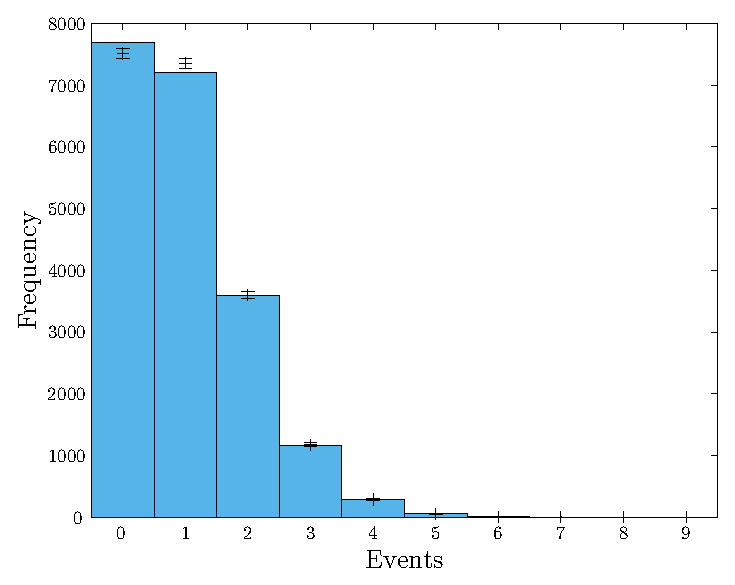
\includegraphics[width=0.6\textwidth]{./images/Fig_Total_event_hist_eLISA}
\caption{Calculated number of detectable EMRBs over a $2\units{yr}$ eLISA mission. The histogram shows the number of events for $2 \times 10^4$ mission realisations. The points show a Poisson distribution with a mean set by $\mathcal{N}_{2\units{yr}}\super{int}$.}
\label{fig:eLISA-Event-no}
\end{figure}
The event rate is lower than for LISA. The MS and WD rates are much reduced. This is because the inner cut-off extends to the limit of detectability. NSs and BHs are less affected by the inner cut-offs, hence their reduction only reflects the loss in sensitivity when switching from LISA to eLISA. The total event rate, being dominated by BHs and NSs, shares a comparable reduction, being around $60\%$ of the LISA rate.

The distribution of SNRs for bursts detectable with eLISA is shown in \figref{SNR-hist-eLISA}.
\begin{figure}%[ht]
\centering
   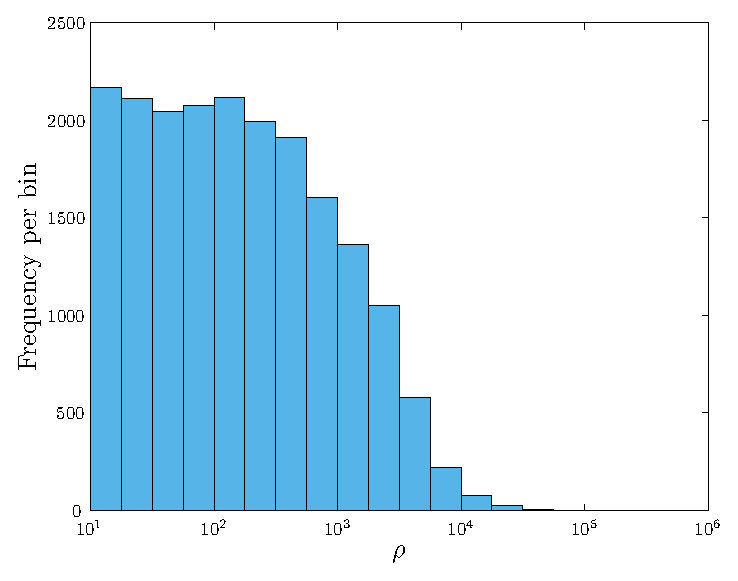
\includegraphics[width=0.6\textwidth]{./images/Fig_Detect_SNR_hist_eLISA}
\caption{Histogram showing the SNR distribution of the detectable bursts from the $2 \times 10^4$ eLISA mission realisations. The bins are uniformly spaced in $\log\rho$ with width $0.25\units{dex}$.}
\label{fig:SNR-hist}
\end{figure}
The median SNR across all the detectable bursts is $\rho \simeq 140$ ($\log\rho \simeq 2.15$). The distribution does not incorporate as many loud events as with LISA and there is a more pronounced decline with increasing SNR. The largest SNR was $\rho \simeq 4.61 \times 10^4$ ($\log\rho \simeq 4.66$).

\subsection{Extragalactic event rate}\label{sec:extragal-events}

As a final event rate calculation, we may consider the question of extragalactic bursts. If we had detailed measurements of the centres of other galaxies, we could adapt our model and generate appropriate rates. However, this would be expensive to do for all galaxies. Instead we reuse our Galactic model, calculating the event rate per Milky Way equivalent galaxy (MWEG), which gives a rough guide for the scaling with the number of galaxies. The event rates estimated are crude, but give a sketch of what we could expect.

In \chapref{extragal}, we found that for the most promising extragalactic sources, EMRBs become informative for $r\sub{p} \lesssim 8 r\sub{g}$. We may use this as an outer cut-off. We only consider bursts from BHs as less massive COs have lower SNRs and so are less informative. The calculated event rate for a $2\units{yr}$ mission is $\mathcal{N}_{2\units{yr}}\super{int} \simeq 0.19$ per MWEG. Therefore, we require the equivalent of approximately five Milky Ways to expect to see one extragalactic burst in a LISA mission lifetime.

\section{Information content}

\subsection{Analysing mission posteriors}

We wish to quantify what we could learn over a mission about the Galactic MBH's mass and spin. We use the parameter set $\boldsymbol{\lambda}_\bullet = \{\ln (M_\bullet/M_\odot), a_\ast, \cos \Theta\sub{K}, \Phi\sub{K}\}$ as each of these has a uniform prior.\footnote{See \secref{Mod-param} for a discussion of these parameters.}

The information carried by a burst is encoded in its posterior probability distribution. This can be recovered using an MCMC as explained in \secref{Estimation}. We ran MCMCs for bursts from the first $100$ of our mission realisations that had periapses $r\sub{p} < 16 r\sub{g}$. There were a total of $96$ interesting bursts ($57$ from BHs and $39$ from NSs) across $63$ missions. %\footnote{NSs are less informative than BHs. The CO mass is degenerate with the distance to the source, hence the extragalactic bursts give an indication of what happens when the CO mass is reduced (although changing from a $10 M_\odot$ BH to a $1.4 M_\odot$ NS is not as extreme as moving to another galaxy).}
Ideally, we would use information from all detectable bursts, but this would be computationally expensive and we do not expect to glean much useful information from orbits with larger periapses.

During an individual mission there may be either zero, one or multiple bursts of interest. In the first case, we learn nothing.\footnote{An absence of bursts does tell us something about the distribution of COs in the NSC; however, with our current state of knowledge, detecting no bursts is not surprising, therefore we have no need to update this.} In the second, we have only to consider the posterior from our MCMC. In the third, we must combine the posteriors of all the bursts. This is easy in theory: as the priors are uniform we have only to multiply the individual posteriors,
\begin{equation}
p(\boldsymbol{\lambda}_\bullet|\{\boldsymbol{s}_i(t)\}\sub{mission}) = \prod_i p(\boldsymbol{\lambda}_\bullet|\boldsymbol{s}_i(t)),
\end{equation}
where $\{\boldsymbol{s}_i(t)\}\sub{mission}$ is the set of bursts for the mission. However, since we have a sampled posterior rather than an analytic function, this is difficult in practice.

The simplest thing to do is bin the points and then multiply the numbers in each bin together (dividing by the area of the bin to convert back to a probability density). The question is then, what is an appropriate bin size? Bins that are too large give insufficient resolution, whilst those that are too small may not encompass any sampled points.

One means of creating bins with sizes that reflect the structure of the distribution is using a $k$-d tree as described in \secref{k-d}. Taking each burst posterior in turn, we construct a $k$-d tree using the two-step method. We use this tree to bin the other posteriors and multiply the totals together. This gives us one estimate for the combined posterior for each of the input bursts. We resample the final distributions (sampling each leaf uniformly) to create sets of points that can be treated in the same way as the output from an MCMC.

\subsection{Distribution widths}

The precision to which a parameter can be constrained may be quantified by the width of the distribution. We use the standard deviation $\sigma\sub{SD}$ and the half-width of the $68$-percentile range constructed from one-dimensional $k$-d trees $\sigma_{0.68}$.

The widths calculated from multiple burst posteriors may be biased to too large values. This can happen when combining distributions of significantly different widths. When using the $k$-d tree of a distribution that is much broader than the others, a small number of leaves can contain the majority of the final posterior probability and we cannot resolve the final width. When using the $k$-d tree from a narrow distribution, there can be large leaves at the edges of the parameter ranges; because the resampled points from these leaves are uniformly distributed, they can skew the overall distribution. Since the bias increases the width, we use the smallest of the calculated values.\footnote{The distributions were checked to ensure that they did not have anomalously small widths due to a computational error.}
In many cases the variation is comparable to the intrinsic scatter from random sampling. The $68$-percentile half-width appears more robust against biasing.

Combining the results from the set of realisations, \figref{Widths} shows the fraction of missions $\mathcal{F}(\sigma > \varsigma)$ that have posterior widths larger than $\varsigma$.
\begin{figure}%[ht]
\centering
   \subfigure[{Logarithm of mass}]{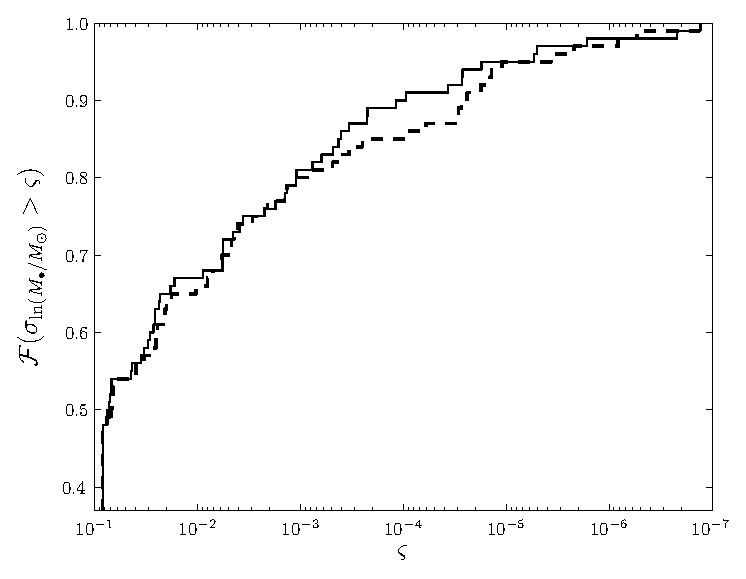
\includegraphics[width=0.475\textwidth]{./images/Fig_mission_sigma_1}} \quad 
   \subfigure[{Spin magnitude}]{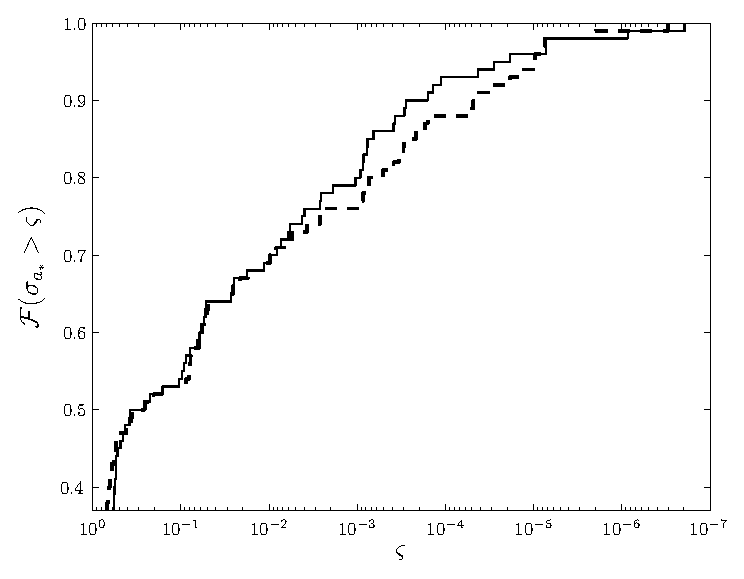
\includegraphics[width=0.475\textwidth]{./images/Fig_mission_sigma_2}} \\
   \subfigure[{Cosine of polar angle}]{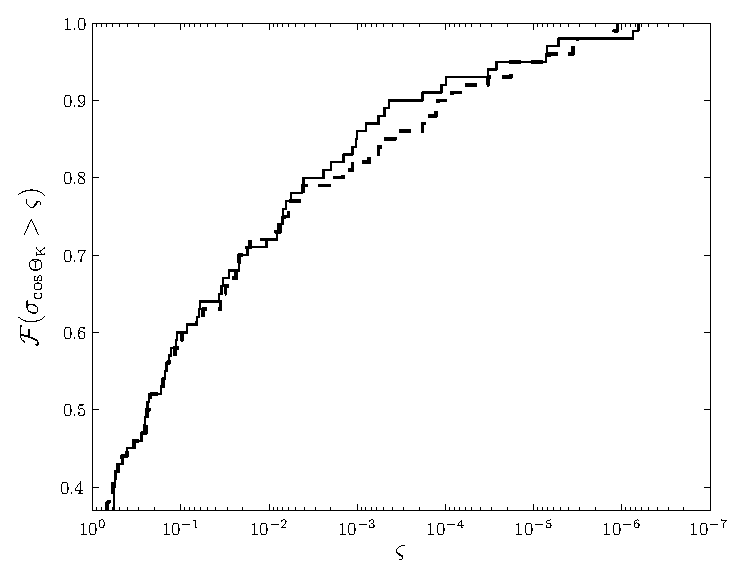
\includegraphics[width=0.475\textwidth]{./images/Fig_mission_sigma_3}} \quad
   \subfigure[{Azimuthal angle}]{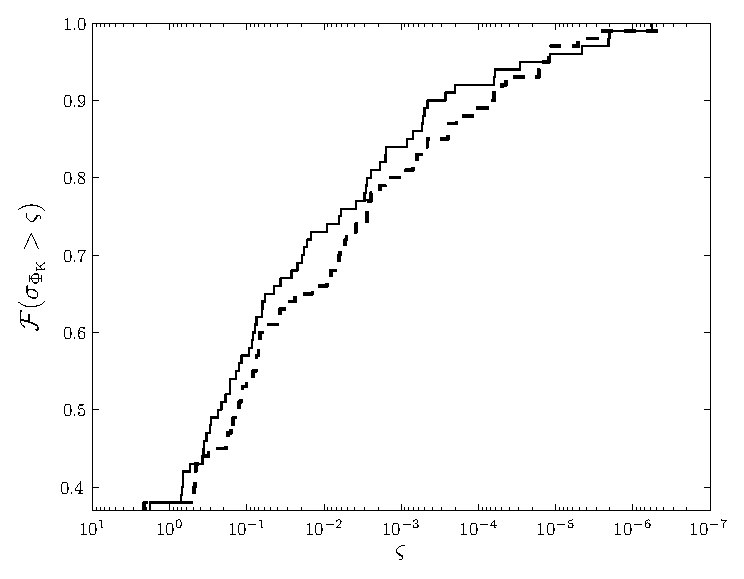
\includegraphics[width=0.475\textwidth]{./images/Fig_mission_sigma_4}}
\caption{Cumulative proportion of mission realisations that produced posteriors with standard deviation (solid line) or $68$-percentile half-width (dashed line) larger than the abscissa value.}\label{fig:Widths}
\end{figure}
It appears that there is a $33\%$ chance of determining $\ln (M_\bullet/M_\odot)$ to a precision of $10^{-2}$ or a $10\%$ chance of determining it to $10^{-4}$. The current uncertainty of $\sim 0.08$ is bettered in over half ($52\%$) of the missions. The spin $a_\ast$ could be determined to a precision of $10^{-2}$ in $30\%$ of missions and there is a $10\%$ chance of determining it to better than $3\times 10^{-4}$.

\subsection{Information entropy}

The distribution widths work for describing parameter estimation accuracies of an individual mission; however, they are less useful for calculating an average since they are undefined when no bursts are detected. There is an alternative means of characterising what we could learn: the information entropy of the posterior distribution.

\citet{Shannon1948,Shannon1948a} introduced the idea of information entropy, which quantifies the expectation for information gained from an outcome or, equivalently, the amount of uncertainty regarding a system \citep[chapters 2 and 4]{MacKay2003}. For a discrete ensemble of probabilities $\{p_i\}$,
\begin{equation}
H(\{p_i\}) = -\sum_i p_i \ln p_i
\end{equation}
is the entropy measured in nats.\footnote{The unit is set by the base of the logarithm; the more familiar bit is calculated using base two, $1\units{bit} \equiv \ln(2)\units{nats}$.} This is identical to its counterpart in statistical physics up to a factor of the Boltzmann constant. Generalising from discrete to continuous probabilities is not quite as simple as exchanging the sum for an integral; it is also necessary to introduce a measure function in the logarithm, otherwise the entropy would not be invariant under a simple parameter rescaling. For a continuous probability distribution $p(\lambda)$, we work in terms of the relative entropy \citep[section 1.4]{Ihara1993}
\begin{equation}
H(p|q) = \intd{}{}{p(\lambda)\ln\left(\dfrac{p(\lambda)}{q(\lambda)}\right)}{\lambda},
\end{equation}
where $q(\lambda)$ is another probability distribution, and we have changed the sign compared to the discrete case so that the entropy is non-negative. The relative entropy, or Kullback--Leibler divergence, measures the difference between distributions and is zero only if $p(\lambda) = q(\lambda)$ everywhere; with $p(\lambda)$ as the posterior and $q(\lambda)$ as the prior, it quantifies the information gained \citep{Kullback1951}.

The relative entropy is perfect for our purpose. It is zero when we do not observe a burst or the burst is uninformative such that we do not learn anything. Otherwise it scales approximately with the (logarithm of the) posterior width, giving an indication of how much could be learnt. For example, if $p(\lambda)$ and $q(\lambda)$ were both uniform distributions, with $p(\lambda)$ having $1/z$ the width of $q(\lambda)$, $H(p|q) = \ln z$; if they were both Gaussian with equal means, and $p(\lambda)$ had $1/z$ the width of $q(\lambda)$, $H(p|q) = \ln z - (1/2)(1 - z^{-2})$.

There is one complication in using the relative entropy. We have used an improper prior for $\ln (M_\bullet/M_\odot)$; it is uniform over the entire real line and so cannot be normalised. As an alternative, we can use a Gaussian with parameters set by the current observations \citep{Gillessen2009}. The relative entropy then compares constraints from bursts with those from observing stellar motions.\footnote{Whilst this is a useful comparison, it does mean that the results are specific to the current state of knowledge and cannot be simply translated should we obtain updated measurements.}

In practice, if we were trying to infer the mass of the MBH, we would combine all our data together to form a best estimate. Then a positive entropy would indicate that the final posterior is narrower than the current observational distribution. We do not incorporate our current knowledge of the MBH mass into our prior here because we are interested in what information is contained in EMRBs alone. Therefore, our posterior from EMRBs can be broader than this observational prior. In this event, the relative entropy can still be positive (since the distributions are different) even though we are not gaining information. In these cases we set the entropy to zero by hand, as we have not improved our relative state of knowledge.\footnote{Bursts that are not informative with regards to the MBH mass are primarily from orbits with $r\sub{p} \gtrsim 8 r\sub{g}$ and have $\rho \lesssim 300$.}

The entropies calculated from multiple burst posteriors may show a similar bias to the distribution widths. This would reduce the value; hence, we use the largest calculated entropy. However, the entropy appears much less sensitive to the choice of the $k$-d tree used for the multiplication than the distribution widths. %The entropies corresponding to the distributions in \figref{bias} differ only by $0.04\units{nats}$, less than $1\%$ of the value.

The entropies are well correlated with the logarithm of the distribution widths as expected. The distributions of the fraction of missions with entropies smaller than a given value are shown in \figref{H-ent}.
\begin{figure}%[ht]
\centering
   \subfigure[{Logarithm of mass}]{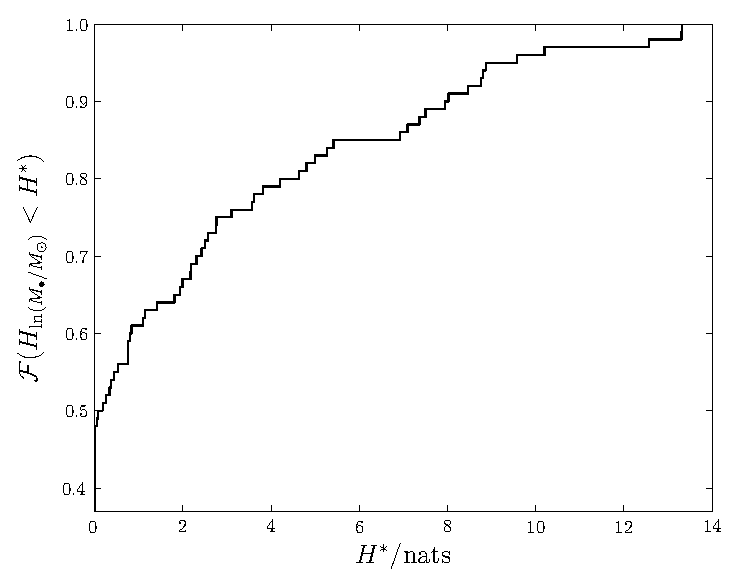
\includegraphics[width=0.475\textwidth]{./images/Fig_mission_entropy_1}} \quad 
   \subfigure[{Spin magnitude}]{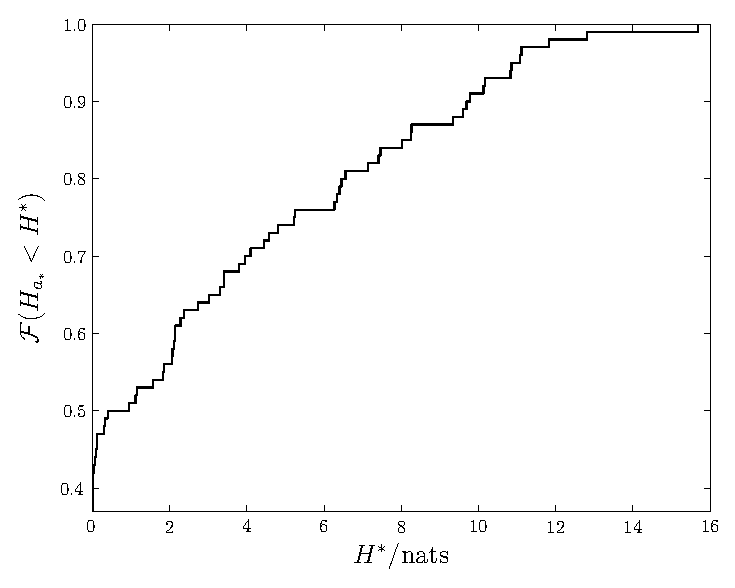
\includegraphics[width=0.475\textwidth]{./images/Fig_mission_entropy_2}} \\
   \subfigure[{Cosine of polar angle}]{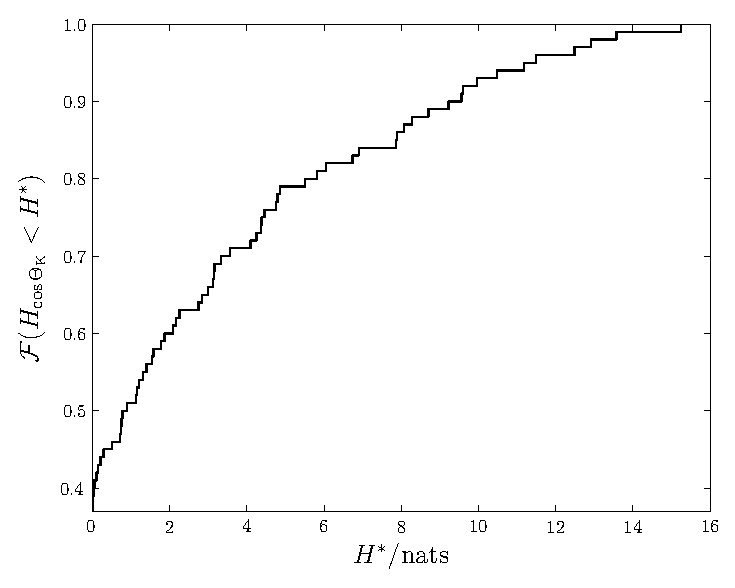
\includegraphics[width=0.475\textwidth]{./images/Fig_mission_entropy_3}} \quad
   \subfigure[{Azimuthal angle}]{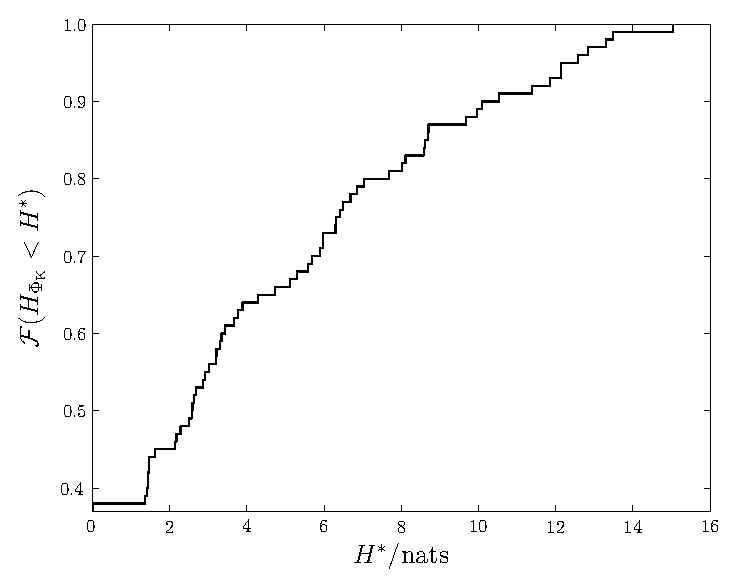
\includegraphics[width=0.475\textwidth]{./images/Fig_mission_entropy_4}}
\caption{Cumulative proportion of mission realisations that produced posteriors with relative entropies larger than the abscissa value. Here, $H_{\lambda_\bullet^a} \equiv H(p(\lambda_\bullet^a)|q(\lambda_\bullet^a))$.}\label{fig:H-ent}
\end{figure}
They closely mirror those in \figref{Widths} (but the scale on the abscissa axis is now linear). There is a clustering at small entropies; the largest entropies are $\sim 13\units{nats}$ for $\ln(M_\bullet/M_\odot)$ and $\sim 15\units{nats}$ for the other parameters.

Taking the average across all $100$ mission realisations, we can calculate the expected information gain for each parameter. The results are shown in \tabref{entropies}
\begin{table}\footnotesize
\centering
  \begin{tabular}{l D{,}{\,\pm\,}{3.3}}
  \toprule
  $\lambda_\bullet^a$ & \multicolumn{1}{c}{$\left\langle H(p(\lambda_\bullet^a)|q(\lambda_\bullet^a))\right\rangle\sub{mission}/\mathrm{nats}$} \\ \midrule
  $\ln(M_\bullet/M_\odot)$ & 2.2 , 0.3 \\
  $a_\ast$ & 3.0 , 0.4 \\
  $\cos\Theta\sub{K}$ & 2.8 , 0.4  \\
  $\Phi\sub{K}$ & 3.7 , 0.4 \\
  \bottomrule
\end{tabular}
  \caption{Relative entropies for each of the four MBH parameters averaged over $100$ mission realisations. The quoted uncertainties are just the standard errors calculated from the scatter of entropies and do not include any of the other uncertainties.}\label{tab:entropies}
\end{table}
The typical entropy is about $3 \units{nats}$; this corresponds to an improvement in the precision to which we know parameters by a factor of approximately $20$.

\section{Discussion of extreme-mass-ratio bursts}\label{sec:EMRB-end}

EMRBs are a potentially interesting signal for a future space-borne GW detector. They could give us insight into the properties of MBHs as well as the distribution of COs that surround them in galactic centres.

We have studied bursts across four chapters. We began in \chapref{waveforms} by constructing NK waveforms for parabolic orbits. These are approximate, but comparison with calculations from BH perturbation theory show that the typical accuracy may be of order $5\%$. The waveforms are the foundation of our subsequent analysis.

In \chapref{param} we used the NK waveforms to characterise the SNR of bursts and the posterior distributions inferred from them. EMRBs can give good constraints on the key parameters describing the Galaxy's MBH if the periapse distance is $r\sub{p} \lesssim 10 r\sub{g}$ assuming a $10 M_\odot$ CO. This would allow us to improve upon the current uncertainty in the mass measurement of $8\%$ \citep{Gillessen2009}; we could also measure the spin magnitude to a precision of better than $0.1$. Hence, Galactic bursts could be a useful astronomical tool.

Following on from this, in \chapref{extragal} we investigated extragalactic bursts. A number of galaxies could produce detectable bursts, most notably M32. From amongst the most promising candidates, we studied M32, NGC 4945 and NGC 4395 in detail. Bursts from these galaxies can be informative if $r\sub{p} \lesssim 8 r\sub{g}$, again assuming a $10 M_\odot$ CO. Therefore, extragalactic EMRBs could also be useful, although not to the same level as Galactic bursts.

For both Galactic and extragalactic bursts, the limiting factor is the event rate. In this chapter we built a simple theoretical model to predict the Galactic EMRB event rate. This is built upon the Fokker--Planck simulations of \citet{Alexander2009} and incorporates approximate treatments of GW inspiral, tidal disruption and collisions. As part of this, it is necessary to calculate the relaxation time-scale. This is done in the following chapter, where we explore the effects of gravitational two-body interactions. The burst event rate is dominated by stellar-mass BHs which form a cusp about the central MBH as a consequence of mass segregation.

For Galactic bursts, we calculate that there could be on average $\sim1.7$ detectable bursts over a $2\units{yr}$ LISA mission lifetime, of which $\sim1.2$ are from BHs. For eLISA, the number of detectable bursts is reduced by $60\%$ giving a total of $\sim1$ events per $2\units{yr}$ mission, of which $0.7$ are from BHs. The number of events scales linearly with the mission lifetime. The event rate is not high: EMRBs shall not be a prolific GW source; however, the rate is not negligible. We are not guaranteed to have a burst in a mission lifetime, but it seems more likely than not that we shall have at least one.

Adapting the model for the GC, we calculated an estimate for the extragalactic rate. Only considering BHs, over a $2\units{yr}$ mission there may be $\sim0.2$ useful bursts per MWEG. Whilst this does not rule out extragalactic bursts as impossible, it does mean that they are unlikely to be plentiful.

The detectability of EMRBs is of little interest astrophysically unless we can extract information about their source systems. We investigated what we could expect to learn about the Galaxy's MBH. We created bursts for $100$ mission realisations and characterised the posterior probability distributions for the MBH's parameters using MCMC sampling. In a large minority ($\sim40\%$) of realisations, we cannot improve upon our existing knowledge. However, in most cases we can, and it may be possible to gain a highly precise measurement of the MBH's mass and spin.

To quantify the information gained during a mission, we used the relative entropy with respect to our current knowledge. Averaging across all the missions, we found that we can expect to gain $2.2\units{nats}$ of information about the logarithm of the mass, $3.0\units{nats}$ about the spin magnitude, $2.8\units{nats}$ about the cosine of the polar angle for the spin axis and $4.2\units{nats}$ about the azimuthal angle. The entropy scales with the logarithm of the width of the posterior distribution; hence, these entropies represent improvements in the precision of our knowledge of the parameters by factors between $\sim9$ and $\sim40$. For the mass, this would mean that the uncertainty would become $\sim1\%$; we could expect to know the spin to a precision of the order of $\sim0.1$.

These results have been obtained assuming the classic LISA design. The first millihertz space-borne interferometer is likely to have a descoped design such as the proposed eLISA. This concept could be revised in the near future and so we have not used it to produce results. The effect of the reduced sensitivity would be to reduce the SNR and increase the widths of the posterior distributions. The information gained about the MBH would decrease; since the event rate for the most informative bursts in largely unaffected, we could still expect to learn something using eLISA.

It must be stressed that, while these results are computed accurately based on the assumptions of the model, they are only to be trusted to an order of magnitude because of the significant uncertainties in the underlying assumptions. There are a number of sources of uncertainty found throughout our analysis. First, we employed the NK approximation, assuming parabolic trajectories. The waveforms are easy to compute, but do contain inaccuracies in their amplitude profiles. This should not significantly influence detectability, but may lead to differences in the shape of the posterior distributions. Since the errors in the waveforms are small, this should not qualitatively affect our results. Second, in calculating the event rate we made both mathematical and physical approximations. The former are correct to a few percent and so are negligible compared to the latter. Our model, however, does include all the relevant physical processes, and further advances the previous work of \citet{Rubbo2006} and \citet{Hopman2007}. Third, the astrophysical parameters used as inputs for our event rate calculation are themselves uncertain. Fourth, when calculating the constraints for our mission realisations, we only considered EMRBs from orbits with periapses smaller than $16 r\sub{g}$, yet whilst little information is expected from other bursts, the amount is not zero. This may lead us to slightly underestimate the total information that could be extracted from EMRBs. Finally, when combining posteriors from multiple EMRBs from the same mission, we binned our posterior distributions. This could lead to a small bias, making us underestimate the usefulness of bursts. Overall, the uncertainty in astrophysical parameters is likely to be the greatest source of error. As there are many unknowns regarding the physical assumptions it is difficult to quantify the uncertainty in our results. As we learn more about the GC, we shall become more confident in our predictions.

The centre of the Galaxy is a wonderful laboratory for testing our understanding of astrophysics, in particular for learning about MBHs and their influence on their environments. EMRBs could be a new means of probing this system.
